% Author: Alvin Thai
%         Nicholas Pelham
% Source: The PGF/TikZ manual

\documentclass{standalone}

\usepackage{pgf}
\usepackage{tikz}
\usetikzlibrary{arrows,automata, positioning}
\usepackage[latin1]{inputenc}

\begin{document}

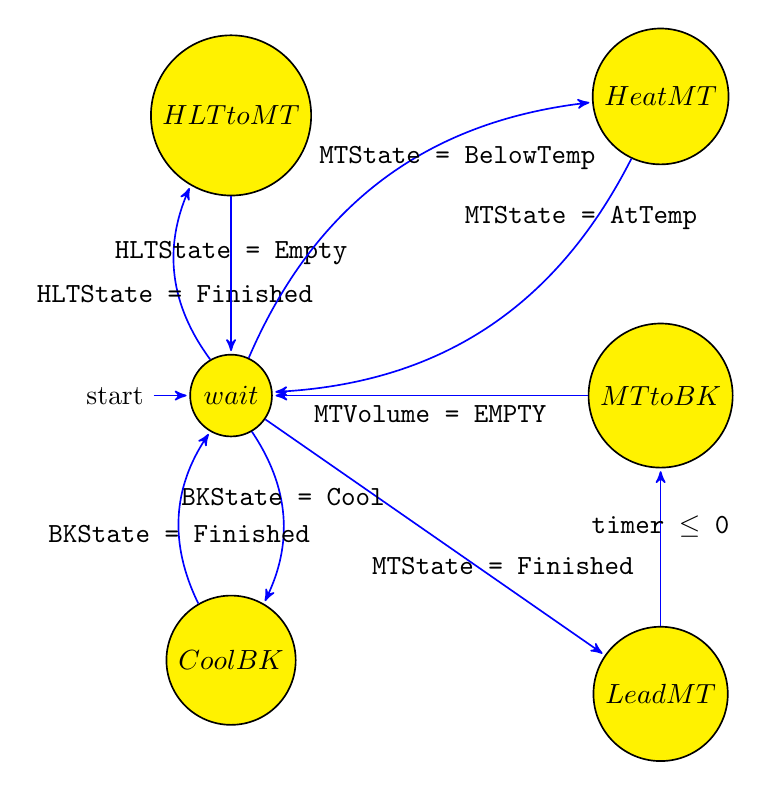
\begin{tikzpicture}[->, >=stealth', shorten >=1pt, auto, node distance=2.8cm,
                    semithick, draw=blue]
  \tikzstyle{every state}=[fill=yellow, draw=black, text=black]

  \node[initial,state] (A) [fill=yellow, draw=black, text=black]    {$wait$};
  \node[state]         (B) [above =2cm of A]                        {$HLTtoMT$};
  \node[state]         (D) [right =4cm of A]                        {$MTtoBK$};
  \node[state]         (C) [above =2cm of D]                        {$HeatMT$};
  \node[state]         (E) [below =2cm of D]                        {$LeadMT$};
  \node[state]         (F) [below =2cm of A]                        {$CoolBK$};

  \path 
        (A) edge [bend left, below, draw=blue]            node {\texttt{HLTState = Finished}} (B)
        (B) edge [above, draw=blue]                       node {\texttt{HLTState = Empty}} (A)
        (A) edge [bend left, below, pos=0.7, draw=blue]   node {\texttt{MTState = BelowTemp}} (C)
        (C) edge [bend left, above, pos=0.2, draw=blue]   node {\texttt{MTState = AtTemp}} (A)
        (A) edge [above, pos=0.7, draw=blue]              node {\texttt{MTState = Finished}} (E)
        (E) edge [above, draw=blue]                       node {\texttt{timer $\leq$ 0}} (D)
        (D) edge [below, draw=blue]                       node {\texttt{MTVolume = EMPTY}} (A)
        (A) edge [bend left, above, draw=blue]            node {\texttt{BKState = Cool}} (F)
        (F) edge [bend left, below, draw=blue]            node {\texttt{BKState = Finished}} (A);
\end{tikzpicture}

\end{document}